\section{\label{sec:level1}Quantum repeater research and development}

\subsection{\label{subsec:level1}Ensemble Collective Encoding}

\begin{figure}[b]
\centering
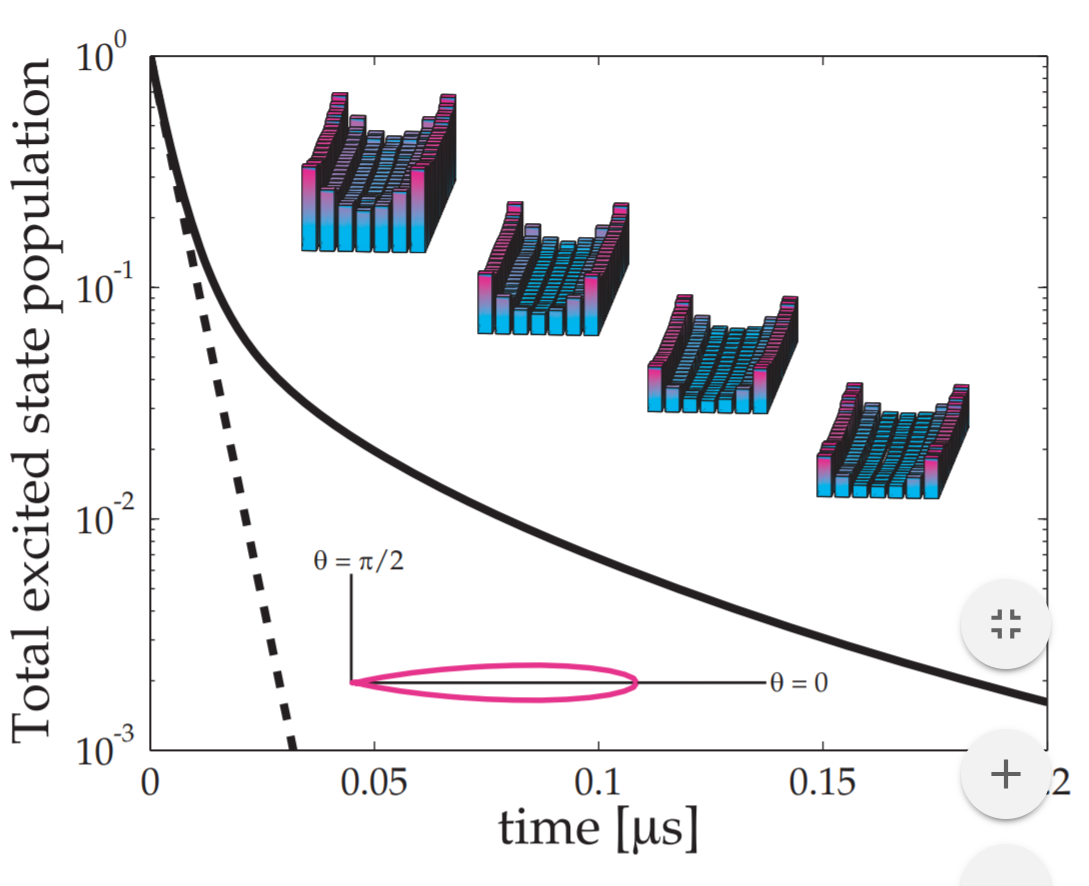
\includegraphics[height=0.32\textwidth,keepaspectratio]{superradiance}
\caption{\label{fig:superradiance} Simulation of the decay of 980 Rydberg excited Rb$^{87}$ atoms is shown by the solid black line. The dashed black line illustrates the $\exp(-2\gamma_{col}t)$ decay rate of a symmetric and super-radiant state. The diagrams represent the distribution of excited state population throughout the ensemble for several layers of the ensemble. The pink cone-shape presents the probability of photon emission as a function of direction at time t=10$^{-7}$s
$^{[}$\citep{Pedersen2009FewEncoding}$^{]}$.}
\end{figure}

\noindent The theoretical research motived by the proposal for collective atomic ensemble excitation, developed in Ref. [\citen{Duan2001Long-distanceOptics}], is discussed in this section. The ability to collectively control the interaction of light with a cloud of N-atoms is two-fold advantageous. The coupling strength scales as $\sqrt{N}$ and therefore increases as the number of atoms in an ensemble increases \citep{Hammerer2010QuantumEnsembles}. Secondly, light emission from an atomic ensemble is in a well-defined direction $^{[}$\citep{Duan2001Long-distanceOptics}$^{]}$.

Furthermore, excitation via Rydberg states enables controlled collective state preparation where the Rydberg blockade mechanism is utilised. The result is a single allowed excitation in an ensemble of atoms where the atom which has been excited is unknown. Pedersen et al. [\citen{Pedersen2009FewEncoding}] investigates collective state encoding and super-radiance through simulation of an ensemble containing a few hundred atoms. The collective superposition atomic state is
\begin{equation}
\label{eq:collectiveencodingstate}
\ket{\Psi_{0}}=1/\sqrt{N}\sum_{j=1}^{N} \exp(i \vec{k}_{0} \cdot \vec{r}_{j})\ket{\textbf{1}_{j}} \otimes \ket{0}_{v},
\end{equation}

\noindent where $\ket{\textbf{1}_{j}}=\ket{0...1_{j}...0}$ is the entangled $\ket{W}$ state and $\ket{0}_{v}$ is the vacuum state. Laser pulses have wavevectors $\vec{k}_{i}$ are used to prepare $\ket{\Psi_{0}}$ such that $\vec{k}_{0}=\sum_{i} \delta_{i}\vec{k}_{i}$. If a photon is absorbed then $\delta_{i}=1$ and if a photon is emitted $\delta_{i}=-1$ $^{[}$\citep{Nielsen2010QuantumInformation}$^{]}$. The collective state evolves such that decay from the excited collective state $\ket{\textbf{1}_{j}}$ produces a photon with wavevector $\vec{k}_{0}$ due to phase matching. 


As shown in Fig.(\ref{fig:superradiance}) the spontaneous emission initially occurs at the rate $\exp(-2\gamma_{col}t)$ depicted by the black dashed line, where $\gamma_{col}$ relates the single atom decay of the Rb$^{87}$ excited state to a multi-atom ensemble. The decreased decay rate beyond 10$^{8}$ s is expected to be due to a loss of symmetry of the excited state population distribution. The emission cone shown in Fig. (\ref{fig:superradiance}) represents 95\% of the photon emission measured within 0.3 rad of $\vec{k}_{0}$. The high directionality of super-radiance emission is a useful tool for coupling to photonic systems and has applications as a single photon source. Additionally, Pedersen et al. $^{[}$\citep{Pedersen2009FewEncoding}$^{]}$ presents the concept of using the internal states of the atomic ensemble as a qubit register. An example of this is shown in Fig. (\ref{fig:qubitregister}b) where the Zeeman sub-levels of Rb$^{87}$ are utilised. Each qubit as shown in Fig.(\ref{fig:qubitregister}a) has a function dependent on the state lifetime. 


\begin{figure}[t]
\centering
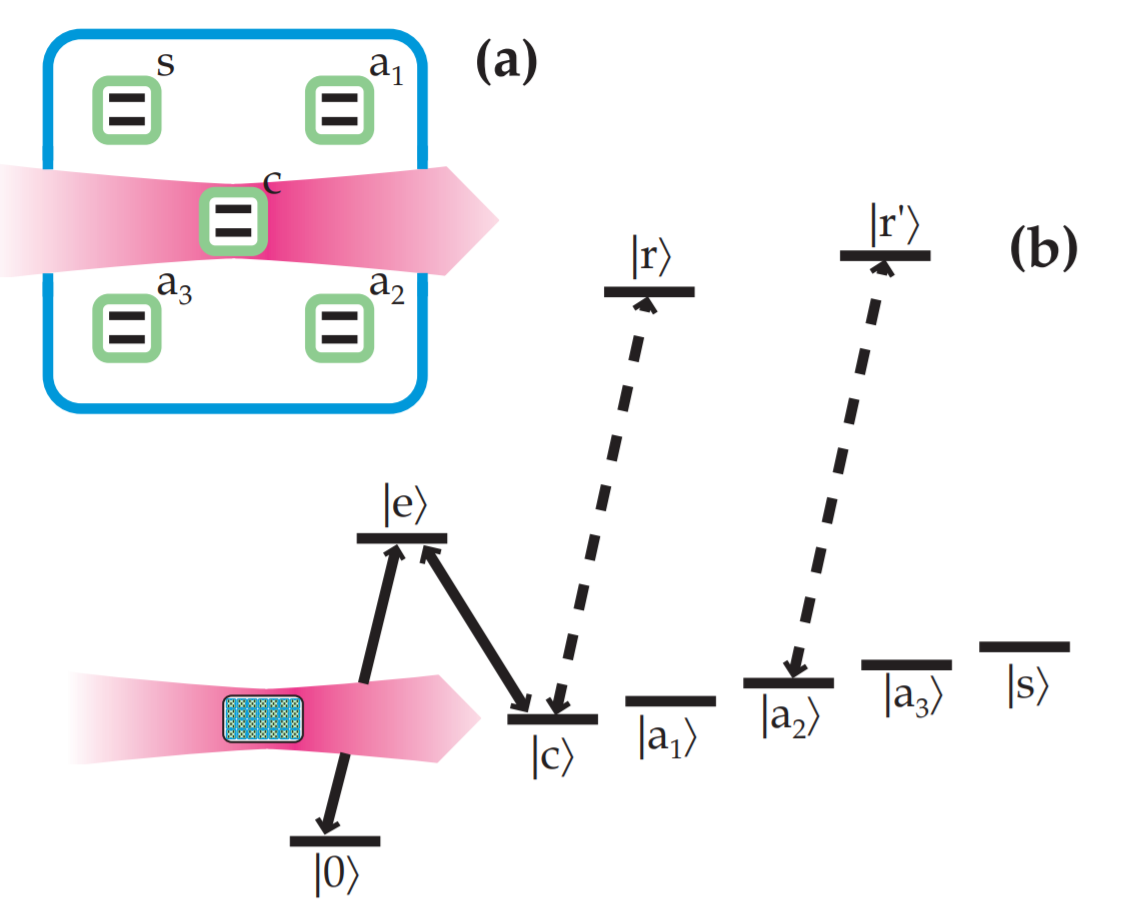
\includegraphics[height=0.32\textwidth,keepaspectratio]{qubitregister}
\caption{\label{fig:qubitregister} (a) five-qubit register contains a storage [s], communication [c] and auxiliary [a1-a3] qubits. (b) Collective internal states of the atomic ensemble $^{[}$\citep{Pedersen2009FewEncoding}$^{]}$.}
\end{figure}



\subsection{\label{subsec:level2}Experimental Demonstration of Collective Encoding}

Experimental observation of the Rydberg blockade effect and collective Fock state encoding of an atomic ensemble is explored in Ref. [\citen{Ebert2014AtomicBlockade}]. An ensemble of 3 $\leq \bar{N} \leq 16$ atoms are initially confined within a magneto-optical trap (MOT). The trap is cooled to ~100 mK temperature to enable the transfer of atoms into a dipole trap. A dipole trap is generated using far-detuned light which induces an atomic dipole moment. The dipole force drives the atom into the minimum of the interaction potential where the distribution of atoms is approximately a Gaussian of length 7 $\mu$m and width < 0.5 $\mu$m $^{[}$\citep{Grimm2000OpticalAtoms,Ebert2014AtomicBlockade}$^{]}$. 

\begin{figure}[t]
\centering
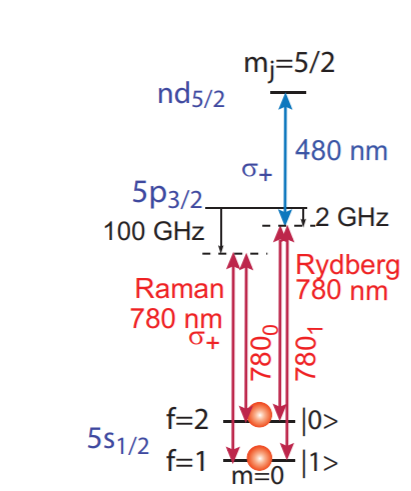
\includegraphics[height=0.32\textwidth,keepaspectratio]{exprimentallaser}
\caption{\label{fig:experimentallaser} Collective ensemble state preparation. The three-level Raman coupling initially prepares the atoms in state $\ket{\textbf{0}}$. Transition to the Rydberg state, $\ket{r}=\ket{nd_{5/2},mf=5/2}$ is competed by 780 nm and 480 nm lasers through two-photon excitation where the lasers and small magnetic field are applied along the z-direction. There is a difference in 780$_{0}$ and 780$_{1}$ to accommodate the Rb$^{87}$ hyperfine ground state splitting. The dipole trap laser is pulsed off during the optical pumping $^{[}$\citep{Ebert2015CoherenceQubits}$^{]}$.}
\end{figure}

\begin{figure}[b]
\centering
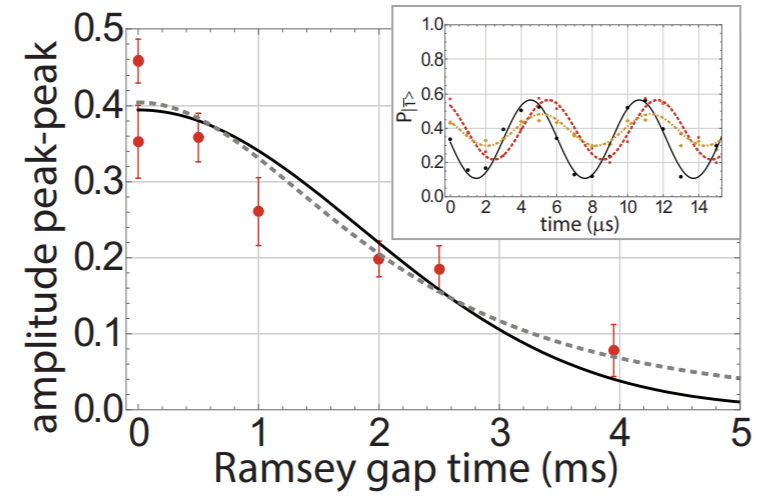
\includegraphics[height=0.32\textwidth,keepaspectratio]{ramseyfringe}
\caption{\label{fig:ramseyfringe} Ramsey interferometry for $\bar{N}=7.6$ to determine the collective qubit coherence time. The peak-peak amplitude as a function of $G(t)$ is measured to obtain $T_{2}=2.63$ by applying a fit model. The fit models $v_{a}$ and $v_{b}$ approximate high and low rates of atomic collisions, respectively $^{[}$\citep{Ebert2015CoherenceQubits}$^{]}$.}
\end{figure}

Two photon-excitation pulses are applied between the Rb$^{87}$ hyperfine ground states $\ket{0},\ket{1}$ to the Rydberg state $\ket{r}$ similarly as described in Fig. (\ref{fig:experimentallaser}). If all atoms are initially in $\ket{\textbf{0}}=\ket{0_{i}...0_{N}}$ the pulse sequence

\begin{equation}
\label{eq:pulsesequence1}
\ket{\textbf{0}} \overrightarrow{\Omega_{N}t=\pi} \ket{\textbf{r}}, \ket{\textbf{r}} \overrightarrow{\Omega t=\pi} \ket{\textbf{1}},
\end{equation}

\noindent prepares $\ket{\Psi_{0}}$ where the collective Rabi frequency is $\Omega_{N}=\sqrt{N}\Omega_{0}$. A circularly polarised beam is applied perpendicular to the pumping beams which acts on atoms in the state $\ket{0}$ to remove atoms from the trap with a fidelity of 97\%. Therefore, ideally the $\mathcal{N}=1$ Fock state is prepared with a fidelity of 62 \%. Prior to ejecting atoms from the dipole trap and careful consideration of the number of atoms residing in each state enables $\mathcal{N} \geq 1$ Fock states to be generated. The atoms residing in $\ket{1}$ are then probed by invoking Rabi oscillations between collective states $\ket{\textbf{1}} \leftrightarrow \ket{\textbf{r}}$ since the known Rabi frequency dependence is $\sqrt{N}$ for N-atoms remaining in the trap. 

Following from the experimental results of Ref. [\citen{Ebert2014AtomicBlockade}], Ebert et al. measured the coherence time of the collective state through a Ramsey interferometry experiment. The Ramsey pulse sequence,

\begin{equation}
\label{eq:pulsesequence1}
R_{1}(\pi)R_{1}(\pi /2)R_{0}(\pi)G(t)R_{1}(\pi)R_{0}(\pi /2),
\end{equation}
  


\noindent ideally maps $\ket{\textbf{0}}$ to $\ket{\textbf{1}}$ where $R_{0(1)}(\theta)$ applies a pulse $\theta$ between energy levels $\ket{0(1)}$ and $\ket{r}$. Fig.(\ref{fig:ramseyfringe}) shows the results of plotting the peak-peak amplitude of the Rabi oscillation obtained as a function of the gap time $G(t)$. The coherence time of $T_{2}=2.63$ ms is extracted for $\bar{N}=7.6$ through fitting to models which describe regimes where dephasing is dominated by  collisions between atoms, $v_{a}$ or rates of low collisions, $v_{b}$. From the data collected it appears atomic collisions are a significant dephasing mechanism. However, other possible sources of dephasing include magnetic field fluctuations and intensity noise of the dipole trap or optical pumping lasers $^{[}$\citep{Saffman2005AnalysisAtoms}$^{]}$. Therefore, the coherence time for atoms in $\mathcal{N} \geq 1$ Fock states were measured using the Ramsey interferometry to determine the relationship $T_{2}=1/\bar{N}$. 


\begin{figure}[t]
\centering
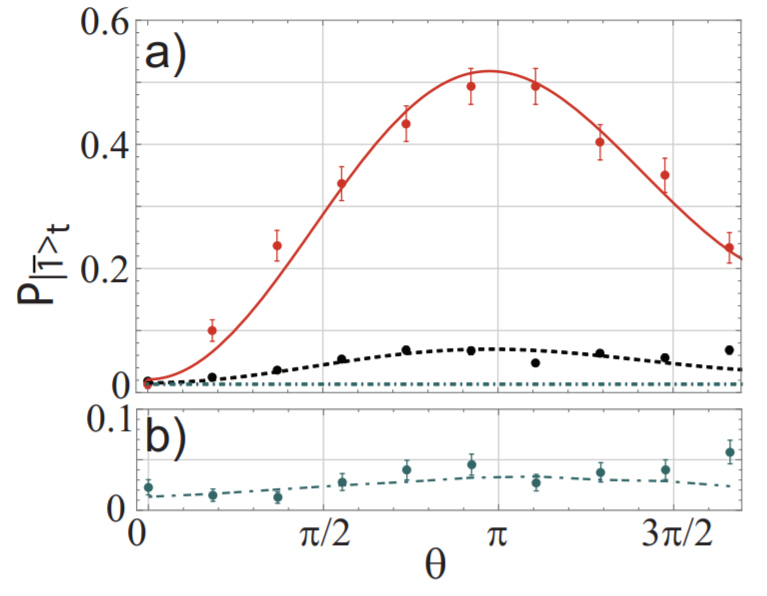
\includegraphics[height=0.37\textwidth,keepaspectratio]{blockadefidelity}
\caption{\label{fig:blockadefidelity} The probability of preparing state $\ket{\textbf{1}}_{t}$ with ($U_{b}$) and without the blockade ($U_{a}$) is shown in black and red, respectively. (b) The estimated 0.3\%/atom contribution of unwanted $\ket{0}_{t}\rightarrow\ket{1}_{t}$ excitation when removing atoms in $\ket{0}$ from the trap is shown by the blue dash-dotted line. Post selection data of $\ket{\textbf{1}}_{c}$ is given by the blue circles $\ket{\textbf{1}}_{c}$ $^{[}$\citep{Ebert2015CoherenceQubits}$^{]}$.}
\end{figure}

\begin{figure}[b]
\centering
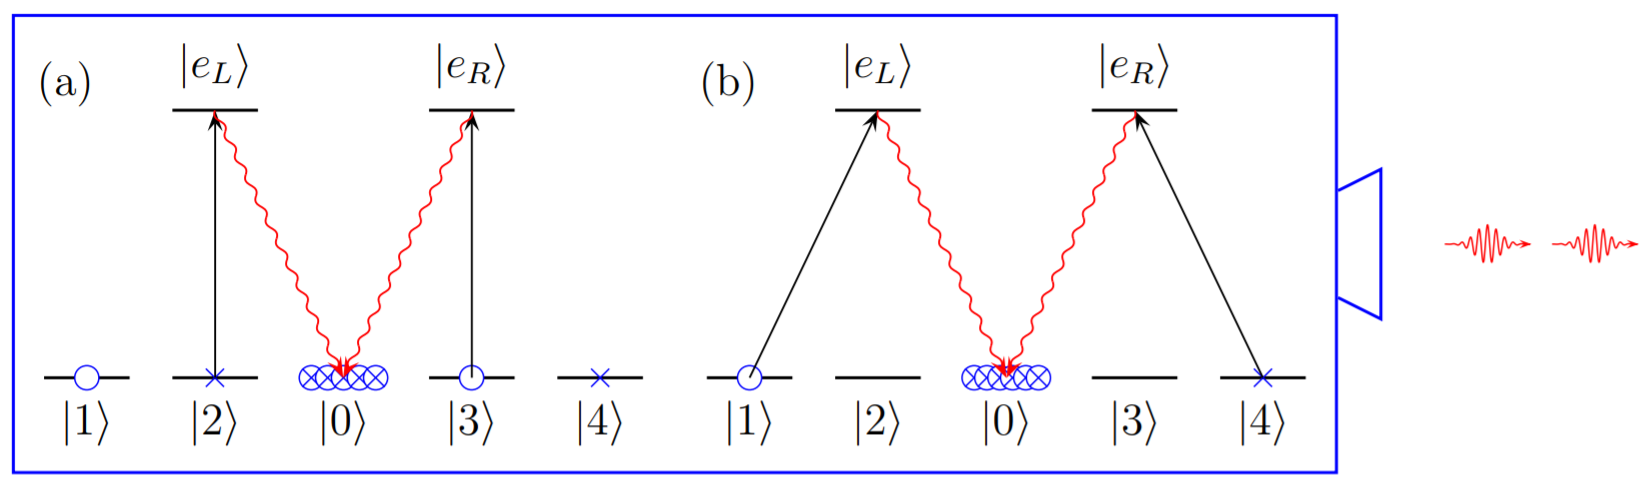
\includegraphics[height=0.13\textwidth,keepaspectratio]{bellstate}
\caption{\label{fig:bellstate} The preparation sequence of a Bell state. (a1) A $\pi$-pulse is applied between $\ket{2} \rightarrow \ket{e_{L}}$ and $\ket{3} \rightarrow \ket{e_{R}}$. Decay from the excited Rydberg states $\ket{e_{R(L)}}$ outputs a $\ket{R(L)}$-polarised state. If there is an atom in state $\ket{3}$ the Rydberg blockade effect can be used to block the transition $\ket{0} \rightarrow \ket{e_{R}} \rightarrow \ket{4}$, similarly for exciting an atom to state $\ket{1}$ from $\ket{0}$ if there is an atom initially in $\ket{2}$. (b) The second correlated photon emission is obtained from applying a $\pi$-pulse between $\ket{1} \rightarrow \ket{e_{L}}$ and $\ket{4} \rightarrow \ket{e_{R}}$. The Bell state emitted is $(\ket{L}_{1}\ket{R}_{2}-\ket{R}_{1}\ket{L}_{2})/\sqrt{2}$ $^{[}$\citep{Nielsen2010DeterministicProcessing}$^{]}$.}
\end{figure}

Demonstration of the fidelity for preparing collective states between two ensembles utilising the Rydberg blockade mechanism is thereafter experimentally investigated $^{[}$\citep{Ebert2015CoherenceQubits}$^{]}$. Atoms are initially loaded into two dipole traps separated $\approx$8.7 $\mu$m along $\vec{x}$ where the optical pumping scheme in Fig.(\ref{fig:experimentallaser}) is applied. Initially the probability $P_{t}$ of preparing the collective state is determined. The superposition state $\ket{\textbf{0}}_{c} \left [ \cos (\theta /2) \ket{\textbf{0}}_{t}-\sin (\theta /2)\ket{\textbf{1}}_{t} \right ]$ is ideally prepared by the pulse sequence,
\begin{equation}
\label{eq:pulsesequence1}
U_{a}\ket{\textbf{0}}_{1,c}\ket{\textbf{0}}_{0,t}=R_{t}(\pi)R_{t}(\theta)\ket{\textbf{0}}_{c}\ket{\textbf{0}}_{t}.
\end{equation}
\noindent The state $\ket{\textbf{1}}_{c}\ket{\textbf{0}}_{t}$ is prepared using the Rydberg blockade mechanism through the sequence,
\begin{equation}
\label{eq:pulsesequence1}
U_{b}\ket{\textbf{0}}_{c}\ket{\textbf{0}}_{t}=R_{1,c}(\pi)R_{1,t}(\pi)R_{0,t}(\theta)R_{0,c}(\pi).
\end{equation}

\noindent The fidelity of the Rydberg blockade is measured as $1-\left [ P_{t}(U_{b})/P_{t}(U_{a}) \right ]=0.89$. The results of applying $U_{a}$ and $U_{b}$ are shown in Fig. (\ref{fig:blockadefidelity}). Post selection of $\ket{\textbf{1}}_{c}$ and removing the 0.3 \% /atom blow-away excitation, presents the ensemble-ensemble Rydberg blockade as approximately perfect. 

\begin{figure}[t]
\centering
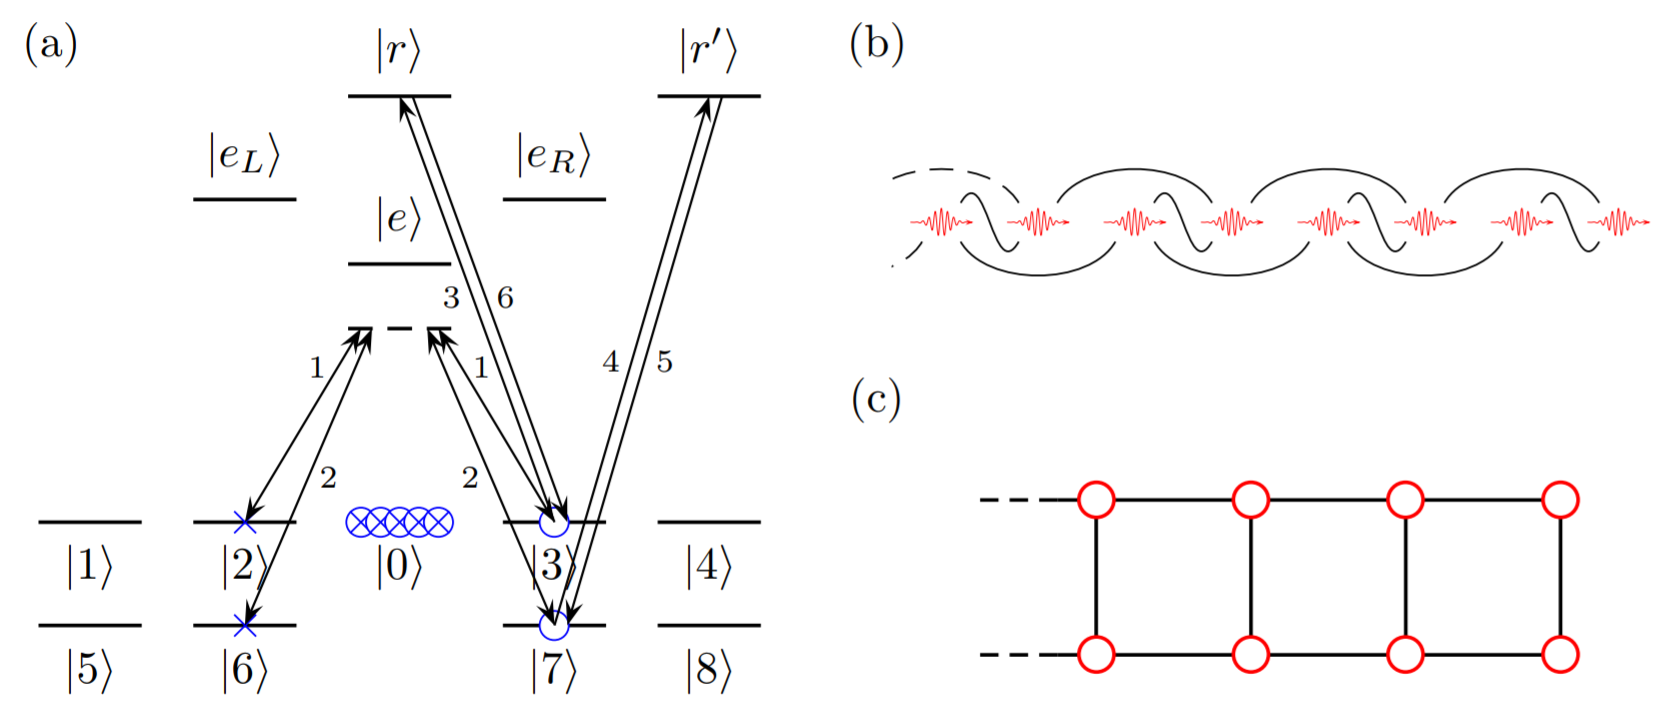
\includegraphics[height=0.20\textwidth,keepaspectratio]{2dimensionalclusterstate}
\caption{\label{fig:2dimensionalclusterstate} Preparation of a 2-dimensional cluster state (a) Following the transition steps and with a single atom initially prepared in $\ket{3}$ and $\ket{7}$. Pulses 1 and 2 apply $\pi/2$ pulse Raman transition and pulses 3-6 apply a $\pi$ rotation and implement Rydberg controlled-phase gates. (b) The first 8 emitted photons and (c) The two-dimensional cluster state $^{[}$\citep{Nielsen2010DeterministicProcessing}$^{]}$.}
\end{figure} 

\subsection{Rydberg entangled state generation}

The presented Rydberg blockade collective state preparation for a single ensemble and between two atomic ensembles is a powerful tool to enable the deterministic generation of entangled states. The Rydberg blockade enables the maximally entangled two-qubit state Bell state, $(\ket{L}_{1}\ket{R}_{2}-\ket{R}_{1}\ket{L}_{2}$, to be generated from a single ensemble where decay from the excited Rydberg states $\ket{e_{R}}$ ($\ket{e_{L}}$) outputs a $\ket{R}$ ($\ket{L}$)-polarised photon \citep{Nielsen2010DeterministicProcessing}. The EPR pairs are used in quantum teleportation, super-dense coding schemes and have correlated measurement outcomes $^{[}$\citep{Nielsen2010QuantumInformation}$^{]}$. Bell state generation is presented in Fig.(\ref{fig:bellstate}) where the initial state $(\ket{0100}-\ket{0010})/\sqrt{2}$ is prepared by transferring a single excitation from $\ket{0}$ to $\ket{2}=\ket{0100}$ and a Raman transition between $\ket{2} \leftrightarrow \ket{3}$.


Fig.(\ref{fig:2dimensionalclusterstate}) illustrates the generation of collective entangled states such as the 2-dimensional cluster state. The 2-dimensional cluster state is generated by connecting two parallel one-dimensional cluster states through a controlled-phase gates. Although Fig. (\ref{fig:2dimensionalclusterstate}) depicts the collective states of single atomic ensemble in Ref.[\citen{Nielsen2010DeterministicProcessing}] it is suggested for this scheme, experimental implementation would be better suited to two atomic ensembles separated a small distance. The GHZ state is expressed as 
\begin{equation}
\label{eq:GHZ}
\ket{GHZ}=\frac{1}{\sqrt{2}}(\ket{+_{i}...+_{N}}_{t}+\ket{-_{i}...-_{N}}_{t}),
\end{equation}
\noindent where $\ket{+(-)}_{t}$ depicts 1 (0) photon emission. To produce the GHZ state initially the pulse sequence $R_{1,c}(\pi)R_{0,c}(\pi/2)$ is applied to $\ket{\textbf{0}}_{c}\ket{\textbf{0}}_{t}$ followed by repeatedly applying $R_{1,t}(\pi)R_{0,t}(\pi)$.  

\subsection{Long-range entanglement}


Long distance entanglement is another requirement to develop a quantum network where the fidelity of an entangled pair in free space decreases exponentially with distance \citep{Sangouard2011QuantumOptics}. Hybrid quantum approaches are considered where Rydberg atomic ensembles provide the qubit memory. Ref. [\citen{Petrosyan2008QuantumResonators}] considers operating a superconducting coplanar waveguide (CPW) at microwave field with atom ensembles place at the field anti-nodes within the cavity. Non-resonant excitation of the atomic ensembles is induced by the cavity frequency $\omega_{c}$ whilst all other modes are far detuned from atomic resonance. The wavelength of the cavity standing wave $\lambda_{c} \approx$4 mm such that the atomic ensembles have a mm-range separation. 

Therefore interaction between the ensembles excited to the Rydberg state is mediated by the van der Waals cavity mode interaction. The presented conditional phase gate scheme, $\ket{s^{x}}_{A}\ket{s^{y}}_{B}\rightarrow (-1)^{xy}\ket{s^{x}}_{A}\ket{s^{y}}_{B}$, is generated between atoms in separate ensembles $A$ and $B$ where $x, y ∈ [0, 1]$. Initially a $\pi/2$ pulse is applied resonant with $\ket{s^{(1)}}\rightarrow\ket{r}_{A,B}$. The gap time is set such that if atoms were initially in $\ket{s^{(1)}}_{A,B}$ they experience an interaction of strength $W$ for time $T_{\pi}=\pi/W$, followed by another $\pi/2$ between $\ket{s^{(1)}}\rightarrow\ket{r}_{A,B}$ to obtain the conditional phase gate.  
\begin{figure}[t]
\centering
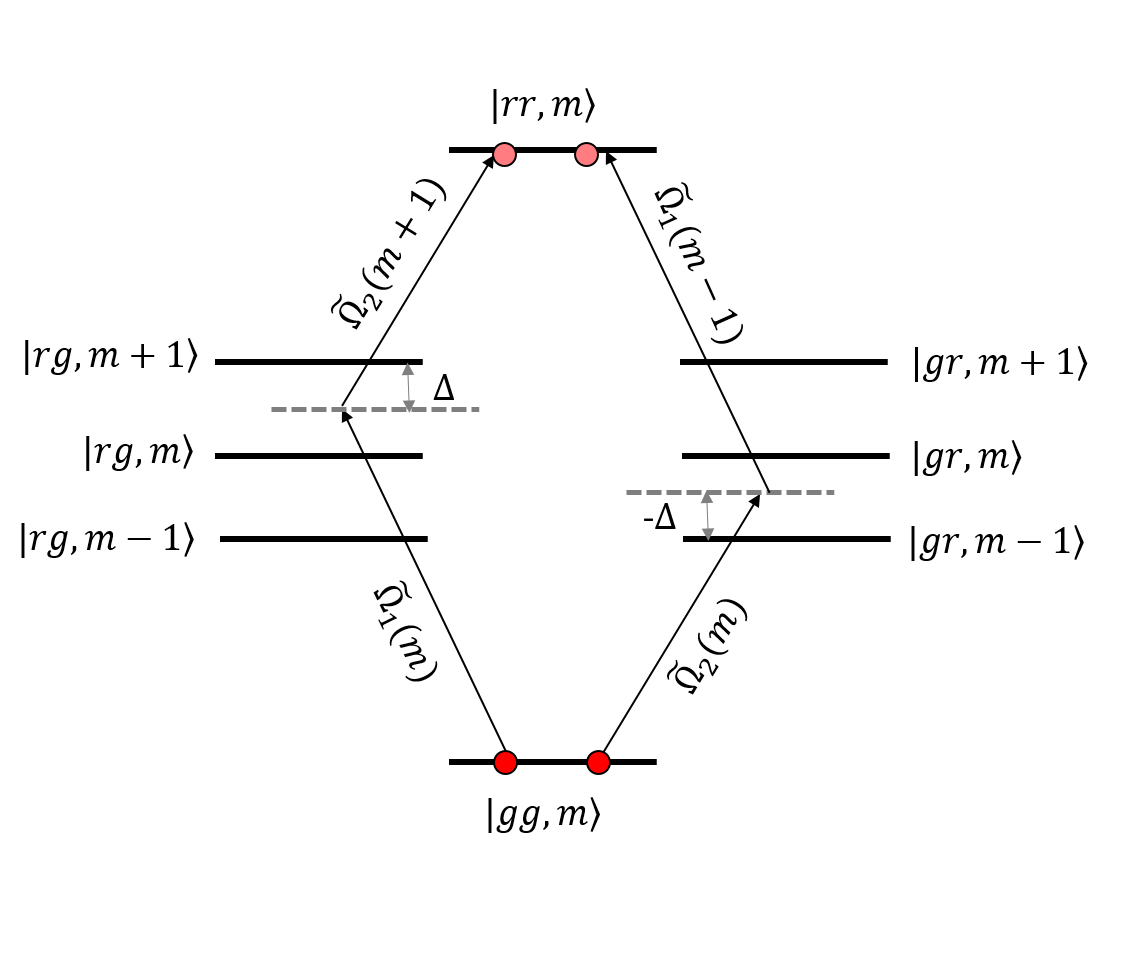
\includegraphics[height=0.32\textwidth,keepaspectratio]{longdistance}
\caption{\label{fig:longdistance} Energy level scheme for enabling pathway excitation for a long distance separation of two atoms in different atomic ensembles.}
\end{figure}

Following from the cavity mediated interaction proposal, Ref. [\citen{Sarkany2015Long-rangeCavity}] presents a long distance entanglement scheme for atoms in different atomic ensembles which is insensitive to thermal photons. This is completed where double excitation from $\ket{gg}\rightarrow \ket{rr}$ can be obtained from two photon cavity field excitation with interfering pathways as shown in Fig. (\ref{fig:longdistance}). Therefore, suppression of the cavity photon number $m$-dependence enables the cavity to operate at a finite temperature, $\approx$4 K, without sacrificing the cavity quality factor $Q$. 

The two-photon resonant collective Rabi frequencies are $\tilde{\Omega}_{1}(n)=\frac{\Omega_{1}g_{a}\sqrt{m+1}}{\delta_{1}}$ and $\tilde{\Omega}_{2}(n)=\frac{\Omega_{2}g_{b}\sqrt{m}}{\delta_{2}}$. The Rabi frequencies replace the two-photon excitation via intermediate states $\ket{a}$ and $\ket{b}$ where $g_{a}$ and $g_{b}$ are the field strength of coupling, respectively. Adiabatic elimination of the intermediate states occurs when $\Omega_{1,2}<<\left | \delta_{1,2}\right |$ where $\delta_{1,2}$ is the detuning of the laser field from the transition $\ket{g}\rightarrow\ket{a,b}$. The choice of $\Omega_{1,2}$ and $\delta_{1,2}$ suppress the $m$-dependence of $\Delta_{1,2}$ derived by perturbation analysis where $\Delta_{1} \approx -\Delta_{2}$. Additionally, the two-photon detuning $\Delta_{1,2}\approx \delta_{1,2}\mp \Delta_{a,b}$ where $\Delta_{a,b}$ is the detuning the cavity field from the atomic transition $\ket{r}\rightarrow \ket{a,b}$ $^{[}$\citep{Sarkany2015Long-rangeCavity}$^{]}$. 


